\documentclass{beamer}  
\usepackage{../slides}
\usepackage{cancel}
\usepackage{appendixnumberbeamer}
\setbeameroption{hide notes}
\defbeamertemplate{description item}{align left}{\insertdescriptionitem\hfill}

%%%%%%%%%%%%%%%%%%%% Not needed at home!
\usepackage[compatibility=false]{caption}
\usepackage{subcaption}
%%%%%%%%%%%%%%%%%%%% Not needed at home!


\title[Binary Regressors]{Mis-Classified, Binary, Endogenous Regressors: Identification and Inference}
\author[FJ DiTraglia]{Francis J.\ DiTraglia\\ Camilo Garc\'{i}a-Jimeno}
\institute{University of Pennsylvania}
\date{September 14th, 2017}
\begin{document} 
%%%%%%%%%%%%%%%%%%%%%%%%%%%%%%%%%%%%%%%%

\begin{frame}[plain]
	\titlepage 
\end{frame} 
%%%%%%%%%%%%%%%%%%%%%%%%%%%%%%%%%%%%%%%%%
\begin{frame}
  \frametitle{Additively Separable Model}
\[
  y = h(T^*, \mathbf{x}) + \varepsilon
\]
\vspace{-1em}
    \begin{itemize}    
    \item $y$ -- Outcome of interest
    \item $h$ -- Known or unknown function 
    \item $T^*$ -- Unobserved, endogenous binary regressor
    \item $T$ -- Observed, mis-measured binary surrogate for $T^*$
    \item $\mathbf{x}$ -- Exogenous covariates
    \item $\varepsilon$ -- Mean-zero error term
    %\item $z$ -- Discrete (typically binary) instrumental variable
  \end{itemize}

\end{frame}
%%%%%%%%%%%%%%%%%%%%%%%%%%%%%%%%%%%%%%%%%
\begin{frame}
  \frametitle{What is the Effect of $T^*$?}
 
  \begin{block}{Re-write the Model}
\begin{align*}
  y &= c(\mathbf{x}) + \beta(\mathbf{x}) T^* + \varepsilon\\
  &\beta(\mathbf{x}) = h(1,\mathbf{x}) - h(0,\mathbf{x})\\
  &c(\mathbf{x}) = h(0,\mathbf{x})
\end{align*}
  \end{block}

  \begin{alertblock}{This Paper:}
    \begin{itemize}
      \item Does a discrete instrument $z$ (typically binary) identify $\beta(\mathbf{x})$? 
      \item What assumptions are required for $z$ and the surrogate $T$?
      \item How to carry out inference for a mis-classified regressor?
    \end{itemize}
  \end{alertblock}
\end{frame}
%%%%%%%%%%%%%%%%%%%%%%%%%%%%%%%%%%%%%%%%%
\begin{frame}
  \frametitle{Example: Job Training Partnership Act (JTPA)}
\framesubtitle{Heckman et al.\ (2000, QJE)}
Randomized offer of job training, but about $30\%$ of those \emph{not} offered also obtain training and about $40\%$ of those offered training don't attend. Estimate causal effect of \emph{training} rather than \emph{offer} of training.

\begin{itemize}
  \item $y$ -- Log wage 
  \item $T^*$ -- True training attendence
  \item $T$ -- Self-reported training attendance
  \item $\mathbf{x}$ -- Individual characteristics
  \item $z$ -- Offer of job training
\end{itemize}
   
\end{frame}
%%%%%%%%%%%%%%%%%%%%%%%%%%%%%%%%%%%%%%%%%%%%
%\begin{frame}
%  \frametitle{Example: Smoking and Birthweight (SNAP Trial)}
%\framesubtitle{Coleman et al.\ (N Engl J Med, 2012)}
%  RCT with 1050 pregnant smokers in England: 521 given nicotine patches, the rest given placebo patches.
%\begin{itemize}
%  \item $y$ -- Birthweight 
%  \item $T^*$ -- True smoking behavior 
%  \item $T$ -- Self-reported smoking behavior
%  \item $\mathbf{x}$ -- Mother characteristics
%  \item $z$ -- Indicator of nicotine patch
%\end{itemize}
%\end{frame}
%%%%%%%%%%%%%%%%%%%%%%%%%%%%%%%%%%%%%%%%%
%\begin{frame}
%  \frametitle{Example: Schooling and Test Scores}
%\framesubtitle{Burde \& Linden (2013, AEJ Applied)}
%  RCT in Afghanistan: 32 villages divided into 11 clusters. Randomly choose 6 and set up school in each village of these clusters.
%
%\begin{itemize}
%  \item $y$ -- Girl's score on math and language test 
%  \item $T^*$ -- Girl's true school attendance
%  \item $T$ -- Parent's report of child's school attendance
%  \item $\mathbf{x}$ -- Child and household characteristics
%  \item $z$ -- School built in village
%\end{itemize}
%\end{frame}
%%%%%%%%%%%%%%%%%%%%%%%%%%%%%%%%%%%%%%%%%%%
%\begin{frame}
%  \frametitle{Example: Returns to Schooling} 
%\framesubtitle{Oreopoulos (2006, AER)}
%Fuzzy RD: minimum school-leaving age in UK increased from 14 to 15 in 1947 but some already stayed until 15 before the law and others failed to comply after it.
%\begin{itemize}
%  \item $y$ -- Log wage 
%  \item $T^*$ -- School attendance at age 15
%  \item $T$ -- Self-report of school attendance at age 15
%  \item $\mathbf{x}$ -- Individual characteristics
%  \item $z$ -- Indicator: born in or after 1933
%\end{itemize}
%   
%\end{frame}
%%%%%%%%%%%%%%%%%%%%%%%%%%%%%%%%%%%%%%%%%%%
\begin{frame}[label=MAHAJAN_BODY]
  \frametitle{Related Literature}
 
  \begin{block}{Continuous Regressor}
    \small
  Lewbel (1997, 2012), Schennach (2004, 2007), Chen et al. (2005), Hu \& Schennach (2008), Song (2015), Hu et al.\ (2015)\ldots 
  \end{block}

  \begin{block}{Binary, Exogenous Regressor}
    \small
   Aigner (1973), Bollinger (1996), Kane et al. (1999), Black et al. (2000), Frazis \& Loewenstein (2003), Mahajan (2006), Lewbel (2007), Hu (2008)
  \end{block}

  \begin{block}{Binary, Endogenous Regressor}
    \alert{Mahajan (2006)}, \small Shiu (2015), Ura (2015), Denteh et al.\ (2016)  
  \end{block}
\end{frame}
%%%%%%%%%%%%%%%%%%%%%%%%%%%%%%%%%%%%%%%
\begin{frame}
  \frametitle{``Baseline'' Assumptions I -- Model \& Instrument}

  \begin{block}{Additively Separable Model}
    $y = c(\mathbf{x}) + \beta(\mathbf{x}) T^* + \varepsilon, \quad \mathbb{E}[ \varepsilon] = 0$ 
  \end{block}

  \begin{block}{Valid \& Relevant Instrument: $z \in \left\{ 0,1 \right\}$}
    \begin{itemize}
      \item $\mathbb{P}(T^*=1|\mathbf{x},z=1) \neq \mathbb{P}(T^*=1|\mathbf{x},z=0)$
      \item $\mathbb{E}[\varepsilon|\mathbf{x},z] = 0$
      \item $0 < \mathbb{P}(z=1|\mathbf{x}) < 1$
    \end{itemize}
  \end{block}

  \begin{alertblock}{If $T^*$ were observed, these conditions would identify $\beta$.}
  \end{alertblock}
\end{frame}
%%%%%%%%%%%%%%%%%%%%%%%%%%%%%%%%%%%%%%%
\begin{frame}
  \frametitle{``Baseline'' Assumptions II -- Measurement Error}


  \begin{alertblock}{Notation: Mis-classification Rates}
    \begin{itemize}
      \item[``$\boldsymbol{\uparrow}$''] 
    $\alpha_0(\mathbf{x},z) \equiv \mathbb{P}\left(T=1|T^*=0,\mathbf{x},z  \right)$
  \item[``$\boldsymbol{\downarrow}$''] 
  $\alpha_1(\mathbf{x},z) \equiv \mathbb{P}\left(T=0|T^*=1,\mathbf{x},z  \right)$
    \end{itemize}
  \end{alertblock}

  \begin{block}{Mis-classification unaffected by $z$}
    $\alpha_0(\mathbf{x},z) = \alpha_0(\mathbf{x}), \quad   \alpha_1(\mathbf{x},z) = \alpha_1(\mathbf{x})$
  \end{block}

  \begin{block}{Extent of Mis-classification}
      $\alpha_0(\mathbf{x}) + \alpha_1(\mathbf{x}) < 1 \quad$ ($T$ is positively correlated with $T^*$)
  \end{block}

  \begin{block}{Non-differential Mis-classification}
     $\mathbb{E}[\varepsilon|\mathbf{x},z,T^*,T] = \mathbb{E}[\varepsilon|\mathbf{x},z, T^*]$
  \end{block}



\end{frame}
%%%%%%%%%%%%%%%%%%%%%%%%%%%%%%%%%%%%%%%
\begin{frame}
  \frametitle{Identification Results from the Literature}

  \begin{block}{Mahajan (2006) Theorem 1, Frazis \& Loewenstein (2003)}
    $\mathbb{E}[\varepsilon|\mathbf{x},z,T^*] = 0$, plus ``Baseline'' $\implies \beta(\mathbf{x})$ identified\\
   \hfill \alert{Requires $(T^*,z)$ jointly exogenous.}
  \end{block}

  \begin{block}{Mahajan (2006) A.2}
    $\mathbb{E}[\varepsilon|\mathbf{x}, z, T^*, T] = \mathbb{E}[\varepsilon|\mathbf{x},T^*]$, plus ``Baseline'' $\implies \beta(\mathbf{x})$ identified\\
    \hfill \alert{Allows $T^*$ endogenous, but we prove this claim is false.}
  \end{block}


  \begin{block}{Open Question}
    Do the baseline assumptions identify $\beta(\mathbf{x})$ when $T^*$ is endogenous?
  \end{block}

\end{frame}
%%%%%%%%%%%%%%%%%%%%%%%%%%%%%%%%%%%%%%%
\begin{frame}
  \frametitle{First-stage Probabilities \& Mis-classification Bounds} 

  \begin{table}[h]
    \centering
  \begin{tabular}[h]{|c|c|}
    \hline
   Unobserved & Observed \\
    $p^*_k(\mathbf{x}) \equiv \mathbb{P}(T^*=1|\mathbf{x}, z=k)$ & 
    $p_k(\mathbf{x}) \equiv \mathbb{P}(T=1|\mathbf{x}, z=k)$\\
    \hline
  \end{tabular}
\end{table}


  \begin{block}{Relationship}
    \vspace{-1em}
   \[
     p_k^*(\mathbf{x}) = \frac{p_k(\mathbf{x}) - \alpha_0(\mathbf{x})}{1 - \alpha_0(\mathbf{x}) - \alpha_1(\mathbf{x})}, \quad k = 0,1
   \]
   \hfill\alert{\footnotesize $z$ does not affect $(\alpha_0, \alpha_1)$; denominator $\neq 0$}
  \end{block}

  \normalsize
  \begin{block}{Bounds for Mis-classification}
    \vspace{-1em}
    \[
      \alpha_0(\mathbf{x}) \leq p_k(\mathbf{x}) \leq 1 - \alpha_1(\mathbf{x}), \quad k = 0,1
    \]
   \hfill \alert{\footnotesize$\alpha_0(\mathbf{x}) + \alpha_1(\mathbf{x}) <1$}
  \end{block}

\end{frame}
%%%%%%%%%%%%%%%%%%%%%%%%%%%%%%%%%%%%%%%
\begin{frame}[plain, c]
  \frametitle{$\alpha_0 \leq \min_k \left\{p_k\right\}, \; \; \alpha_1 \leq \min_k \left\{1 - p_k\right\}$}
\begin{figure}[h]
  \centering
  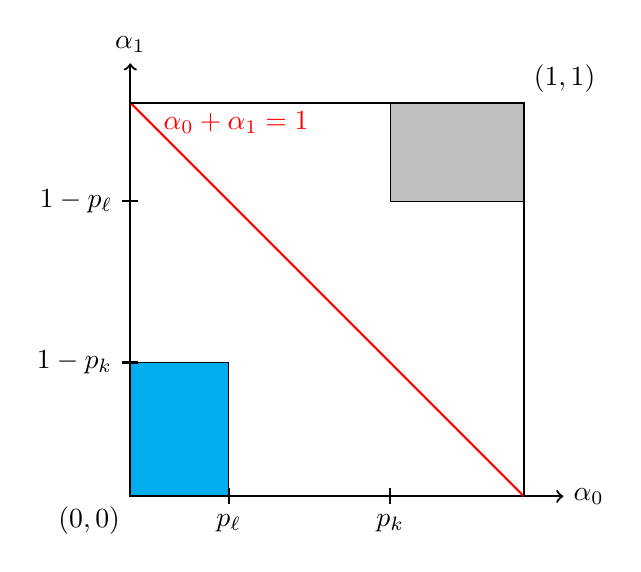
\begin{tikzpicture}[scale=5]
    \draw [fill = lightgray] (0.66,0.75) rectangle (1,1);
    \draw [fill = cyan] (0,0) rectangle (0.25, 0.34);
    \draw [thick, <->] (0,1.1)
    node[above] {$\alpha_1$} -- (0,0) 
    node [below left] {$(0,0)$} -- (1.1,0) 
    node [right] {$\alpha_0$};
    \draw [thick] (0.25,0.02) -- (0.25,-0.02) node [below] {$p_\ell$}; 
    \draw [thick] (0.02,0.75) -- (-0.02,0.75) node [left] {$1 - p_\ell$}; 
    \draw [thick] (0.66,0.02) -- (0.66,-0.02) node [below] {$p_k$}; 
    \draw [thick] (0.02,0.34) -- (-0.02,0.34) node [left] {$1 - p_k$}; 
    \draw [thick, red] (0,1) to (1,0); 
    \node [right, red] at (0.06,0.95) {$\alpha_0 + \alpha_1 = 1$};
    \draw [thick] (0,1) -- (1,1) -- (1,0);
    \node [above right] at (1,1) {$(1,1)$};
    \end{tikzpicture}
\end{figure}
\end{frame}
%%%%%%%%%%%%%%%%%%%%%%%%%%%%%%%%%%%%%%
\begin{frame}
  \frametitle{Instrumental Variable Estimands}
  \begin{block}{Unobserved}
  \[
    \beta(\mathbf{x}) = \frac{\mathbb{E}[y|\mathbf{x},z=1] - \mathbb{E}[y|\mathbf{x},z=0]}{p^*_1(\mathbf{x}) - p^*_0(\mathbf{x})} 
  \]
  \end{block}

  \begin{block}{Wald (Observed)}
    \vspace{-1em}
    \small
    \[
      \frac{\mathbb{E}[y|\mathbf{x},z=1] - \mathbb{E}[y|\mathbf{x},z=0]}{p_1(\mathbf{x}) - p_0(\mathbf{x})} = \beta(\mathbf{x})\left[ \frac{p_1^*(\mathbf{x}) - p_0^*(\mathbf{x})}{p_1(\mathbf{x}) - p_0(\mathbf{x})} \right] = \alert{\frac{\beta(\mathbf{x})}{1 - \alpha_0(\mathbf{x}) - \alpha_1(\mathbf{x})} }
    \]
   
    \vspace{2em}
    \scriptsize
    \[
      \boxed{p_1^*(\mathbf{x}) - p_0^*(\mathbf{x}) = \frac{p_1(\mathbf{x}) - \alpha_0(\mathbf{x})}{1 - \alpha_0 - \alpha_1(\mathbf{x})} -   \frac{p_0(\mathbf{x}) - \alpha_0(\mathbf{x})}{1 - \alpha_0 - \alpha_1(\mathbf{x})} = \frac{p_1(\mathbf{x}) - p_0(\mathbf{x})}{1 - \alpha_0(\mathbf{x}) - \alpha_1(\mathbf{x})}}
    \]
  \end{block}
\end{frame}
%%%%%%%%%%%%%%%%%%%%%%%%%%%%%%%%%%%%%%
\begin{frame}
  \frametitle{Partial Identification Bounds for $\beta(\mathbf{x})$}

    \footnotesize
    \[
      \boxed{ \beta(\mathbf{x}) = \left[ 1 - \alpha_0(\mathbf{x}) - \alpha_1(\mathbf{x}) \right] 
     \left[\frac{\mathbb{E}\left[y|\mathbf{x},z=1\right] - \mathbb{E}\left[y|\mathbf{x},z=0\right]}{p_1(\mathbf{x}) - p_0(\mathbf{x})}\right] }
    \]

    \footnotesize
    \[
      \boxed{ 0 \leq \alpha_0 \leq \min_k \{p_k(\mathbf{x})\}, \quad 0 \leq \alpha_1 \leq \min_k \{1 - p_k(\mathbf{x})\}}
    \]

    \normalsize
    \begin{block}{No Mis-classification}
      $\alpha_0(\mathbf{x}) =  \alpha_1(\mathbf{x}) = 0 \implies \alert{\beta(\mathbf{x}) = }$ \alert{Wald}
    \end{block}

    \begin{block}{Maximum Mis-classification}
      $\alpha_0(\mathbf{x}) = p_{\min}(\mathbf{x}), \, \alpha_1(\mathbf{x}) = 1 - p_{\max}(\mathbf{x})$

      \vspace{-0.5em}
      \begin{align*}
        \implies 1 - \alpha_0(\mathbf{x}) - \alpha_1(\mathbf{x}) = p_{\max}(\mathbf{x}) - p_{\min}(\mathbf{x})
      = |p_1(\mathbf{x}) - p_0(\mathbf{x})|\\
      \implies \alert{\beta(\mathbf{x}) =\mbox{sign}\left\{ p_1(\mathbf{x}) - p_0(\mathbf{x}) \right\}\times (\mbox{Reduced Form})}
    \end{align*}
      
    \end{block}
  
\end{frame}
%%%%%%%%%%%%%%%%%%%%%%%%%%%%%%%%%%%%%%
\begin{frame}
  \frametitle{Partial Identification Bounds for $\beta(\mathbf{x})$}

    \begin{block}{No Mis-classification}
      $\beta(\mathbf{x}) = $ Wald 
    \end{block}

    \begin{block}{Maximum Mis-classification}
      \vspace{-1.5em}
      \begin{align*}
        \beta(\mathbf{x}) &=\mbox{sign}\left\{ p_1(\mathbf{x}) - p_0(\mathbf{x}) \right\}\times (\mbox{Reduced Form})\\
        &=\mbox{sign}\left\{ \mbox{Wald} \right\} \times |\mbox{Reduced Form}|
      \end{align*}
      
      \vspace{1em}
    \footnotesize Wald $> 0\iff \mbox{sign}\left\{ p_1(\mathbf{x}) - p_0(\mathbf{x}) \right\} = \mbox{sign}\left\{ \mbox{Reduced Form} \right\}$ \\
    \footnotesize Wald $< 0\iff \mbox{sign}\left\{ p_1(\mathbf{x}) - p_0(\mathbf{x}) \right\} \neq \mbox{sign}\left\{ \mbox{Reduced Form} \right\}$ 
    \end{block}

    \vspace{1em}
    \begin{alertblock}{
        $\beta(\mathbf{x})$ has the same sign as the Wald and its magnitude is between that of Wald and Reduced Form.}
    \end{alertblock}

\end{frame}
%%%%%%%%%%%%%%%%%%%%%%%%%%%%%%%%%%%%%%
\begin{frame}
  \frametitle{Sharp Bounds?}

  \begin{itemize}
    \item Bounds from the preceding slide are known in the literature.
    \item We prove that they are \emph{not} sharp under the baseline assumptions from above.
      \item $\mathbb{E}[\varepsilon|\mathbf{x},T^*,T,z] = \mathbb{E}[\varepsilon|\mathbf{x},T^*,z]$ restricts $(\alpha_0,\alpha_1)$ hence $\beta$.
    \item Description of the sharp set is somewhat complicated\dots
    \item Corollary: $\beta$ is not point identified regardless of how many (discrete) values $z$ takes on.
  \end{itemize}

  \begin{alertblock}{Point identification from slightly stronger assumptions?}
  \end{alertblock}

\end{frame}
%%%%%%%%%%%%%%%%%%%%%%%%%%%%%%%%%%%%%%
\begin{frame}
  \frametitle{Point Identification: 1st Ingredient}


  \vspace{-1em}

  \begin{block}{Reparameterization}
    \vspace{-1em}
\begin{align*}
  \theta_1(\mathbf{x}) &= \beta(\mathbf{x})/\left[ 1 - \alpha_0(\mathbf{x}) - \mathbf{\alpha}_1(\mathbf{x})  \right]\\
  \theta_2(\mathbf{x}) &= \left[\theta_1(\mathbf{x})\right]^2 \left[ 1 + \alpha_0(\mathbf{x}) - \alpha_1(\mathbf{x})\right] \\
  \theta_3(\mathbf{x}) &= \left[\theta_1(\mathbf{x})\right]^3\left[ \left\{ 1 - \alpha_0(\mathbf{x}) - \alpha_1(\mathbf{x}) \right\}^2 + 6\alpha_0(\mathbf{x})\left\{ 1 - \alpha_1(\mathbf{x}) \right\} \right]
\end{align*}

\[\boxed{\beta(\mathbf{x}) = 0 \iff \theta_1(\mathbf{x}) = \theta_2(\mathbf{x}) = \theta_3(\mathbf{x}) = 0}\]
  \end{block}

  \vspace{-1.5em}

  \begin{block}{Lemma}
    Baseline Assumptions $\implies \alert{\mbox{Cov}(y,z|\mathbf{x}) = \theta_1(\mathbf{x}) \mbox{Cov}(z,T|\mathbf{x})}$.
  \end{block}

\end{frame}
%%%%%%%%%%%%%%%%%%%%%%%%%%%%%%%%%%%%%%
\begin{frame}
  \frametitle{Point Identification: 2nd Ingredient}

  \begin{block}{Assumption (\spadesuit)}
    $\mathbb{E}[\varepsilon^2|\mathbf{x},z] = \mathbb{E}[\varepsilon^2|\mathbf{x}]$
  \end{block}

  \begin{block}{Lemma}
    (Baseline) + (\spadesuit) $\implies$ 
    \[
      \alert{\mbox{Cov}(y^2,z|\mathbf{x}) = 2\mbox{Cov}(yT,z|\mathbf{x}) \theta_1(\mathbf{x}) -\mbox{Cov}(T,z|\mathbf{x})\theta_2(\mathbf{x})}
    \]
  \end{block}

  \begin{block}{Corollary}
    (Baseline) + (\spadesuit) + $[\beta(\mathbf{x})\neq 0] \implies \left[ \alpha_1(\mathbf{x}) - \alpha_0(\mathbf{x}) \right]$ is identified. Hence, $\beta(\mathbf{x})$ is identified if mis-classification is one-sided.
  \end{block}
    

  
\end{frame}
%%%%%%%%%%%%%%%%%%%%%%%%%%%%%%%%%%%%%%
\begin{frame}
  \frametitle{Point Identification: 1st Ingredient}

  \begin{block}{Assumption (\clubsuit)}
    \begin{enumerate}[(i)]
    \item $\mathbb{E}[\varepsilon^2|\mathbf{x},z,T^*,T] = \mathbb{E}[\varepsilon^2|\mathbf{x},z, T^*]$
    \item $\mathbb{E}[\varepsilon^3|\mathbf{x},z] = \mathbb{E}[\varepsilon^3|\mathbf{x}]$
  \end{enumerate}
  \end{block}
 
  \begin{block}{Lemma}
    (Baseline) + (\spadesuit) + (\clubsuit) $\implies$ 
  \small
\[
  \alert{\mbox{Cov}(y^3,z|\mathbf{x}) = 3 \mbox{Cov}(y^2T,z|\mathbf{x}) \theta_1(\mathbf{x}) -3\mbox{Cov}(yT,z|\mathbf{x}) \theta_2(\mathbf{x}) + \mbox{Cov}(T,z|\mathbf{x}) \theta_3(\mathbf{x})}
\]
\end{block}
\end{frame}
%%%%%%%%%%%%%%%%%%%%%%%%%%%%%%%%%%%%%%
\begin{frame}
  \frametitle{Point Identification Result}

  \small 

  \begin{alertblock}{Theorem}
    (Baseline) + (\spadesuit) + (\clubsuit) $\implies \beta(\mathbf{x})$ is point identified.
    If $\beta(\mathbf{x}) \neq 0$, then $\alpha_0(\mathbf{x})$ and $\alpha_1(\mathbf{x})$ are likewise point identified.
  \end{alertblock}

  \begin{alertblock}{Proof Sketch}
    \vspace{-0.5em}
    \begin{enumerate}
      \item $\beta(\mathbf{x})=0 \iff \theta_1(\mathbf{x}) =0$ so suppose this is not the case.  
      \item Lemmas: full-rank linear system in $\theta_1(\mathbf{x}), \theta_2(\mathbf{x}), \theta_3(\mathbf{x})$ \& observables.
      \item Non-linear eqs.\ relating $\theta_1(\mathbf{x}),\theta_2(\mathbf{x}), \theta_3(\mathbf{x})$ to  $\beta(\mathbf{x})$ and $\alpha_0(\mathbf{x}), \alpha_1(\mathbf{x})$. 
        Show that solution exists and is unique.
    \end{enumerate}
  \end{alertblock}

  \vspace{-0.5em}

  \begin{block}{Sufficient Conditions for (\spadesuit) and (\clubsuit)}
    \vspace{-0.5em}
    \begin{enumerate}[(i)]
      \item $T$ is conditionally independent of $(\varepsilon,z)$ given $(T^*,\mathbf{x})$
      \item $z$ is conditionally independent of $\varepsilon$ given $\mathbf{x}$
    \end{enumerate}
  \end{block}
  
\end{frame}
%%%%%%%%%%%%%%%%%%%%%%%%%%%%%%%%%%%%%%
\begin{frame}
  \frametitle{Just-Identified GMM Estimator: Part I}
  \framesubtitle{Suppress dependence on $\mathbf{x}$ to simplify the notation from here on\dots}

  \begin{block}{Collect Lemmas from Above:}
\small
\vspace{-2em}
\begin{align*}
  \mbox{Cov}(y,z) - \mbox{Cov}(T,z) \theta_1 &= 0\\
  \mbox{Cov}(y^2,z) - 2\mbox{Cov}(yT,z) \theta_1 + \mbox{Cov}(T,z)\theta_2 &= 0\\
  \mbox{Cov}(y^3,z) - 3 \mbox{Cov}(y^2T,z) \theta_1 + 3\mbox{Cov}(yT,z) \theta_2 - \mbox{Cov}(T,z) \theta_3 &= 0
\end{align*}
\end{block}

\begin{block}{Notation: Observed Data Vector}
  \vspace{-1.5em}
  \[
\mathbf{w}_i' = (T_i, y_i, y_iT_i, y_i^2, y_i^2 T_i, y_i^3)
\]
\end{block}
\end{frame}
%%%%%%%%%%%%%%%%%%%%%%%%%%%%%%%%%%%%%%%%%%%%%%%
\begin{frame}
  \frametitle{Just-Identified GMM Estimator: Part II}

\[
\boxed{\mathbb{E}\left[
  \big(\boldsymbol{\Psi}'(\boldsymbol{\theta})\mathbf{w}_i - \boldsymbol{\kappa}\big) \otimes 
\left(
\begin{array}{c}
  1 \\ z_i
\end{array}\right)
\right] = \mathbf{0}}
\]

\footnotesize
\begin{align*}
\boldsymbol{\Psi} &= \left[
  \begin{array}{ccc}
    \boldsymbol{\psi}_1 & \boldsymbol{\psi_2} & \boldsymbol{\psi_3}
\end{array}\right]
& \boldsymbol{\kappa} &= (\kappa_1, \kappa_2, \kappa_3)' \equiv \mbox{ ``Intercepts''}\\
  \boldsymbol{\psi}_1' &= \left[
  \begin{array}{cccccc}
-\theta_1 & 1 & 0 & 0 & 0 & 0
  \end{array}
\right] & \theta_1 &= \beta / (1 - \alpha_0 - \alpha_1)\\
  \boldsymbol{\psi}_2' &= \left[
  \begin{array}{cccccc}
\theta_2& 0& -2\theta_1& 1& 0& 0
  \end{array}
\right] & \theta_2 &= \theta_1^2 \left[ 1 + \alpha_0 - \alpha_1 \right]\\
  \boldsymbol{\psi}_3' &= \left[
  \begin{array}{cccccc}
-\theta_3& 0& 3\theta_2& 0& -3\theta_1& 1
  \end{array}
\right] & \theta_3 &= \theta_1^3 \left[ \left( 1 - \alpha_0 - \alpha_1 \right)^2 + 6\alpha_0 (1 - \alpha_1) \right] 
\end{align*}

\begin{alertblock}{Weak Identification Problem}
  Moment conditions are uninformative about $(\alpha_0,\alpha_1)$ when $\beta$ is small.
  Moreover, $(\alpha_0,\alpha_1)$ could be on the boundary of the parameter space.
\end{alertblock}

%\begin{align*}
%\kappa_1 &= c - \alpha_0 \theta_1\\
%  \kappa_2 &= c^2 + \sigma_{\varepsilon\varepsilon} + \alpha_0 (\theta_2 - 2c \theta_1)\\
%  \kappa_3 &= c^3 + 3\left( c - \theta_1 \alpha_0 \right) \sigma_{\varepsilon\varepsilon} + \mathbb{E}[\varepsilon^3] - \alpha_0 \theta_3 - 3 c \alpha_0 \left[ \theta_1 \left( c + \beta \right) - 2\theta_1^2 (1 - \alpha_1) \right]
%\end{align*}


\end{frame}
%%%%%%%%%%%%%%%%%%%%%%%%%%%%%%%%%%%%%%
\begin{frame}
  \frametitle{Weak Identification Problem}

\begin{itemize}
  \item $\beta$ small $\Rightarrow$ moment equalities uninformative about $\alpha_1$
  \item Same problem for other estimators from the literature but hasn't been pointed out.
  \item Identification robust inference: GMM Anderson-Rubin statistic
  \item \alert{But we can do better\ldots}
    \item Bounds for $(\alpha_0, \alpha_1)$ immune to weak identification problem: remain informative if $\beta$ is small or zero.
    \item Inference using Generalized Moment Selection (Andrews \& Soares, 2010)
\end{itemize}


\end{frame}

%%%%%%%%%%%%%%%%%%%%%%%%%%%%%%%%%%%%%

\begin{frame}
  \frametitle{Inference With Moment Equalities and Inequalities}
  \small

\begin{block}{Moment Conditions}
  $\mathbb{E} \left[ m_j(\mathbf{w}_i,\vartheta_0) \right] \geq 0, \quad j = 1, \cdots, p$\\
  $\mathbb{E} \left[ m_j(\mathbf{w}_i,\vartheta_0) \right]  = 0, \quad j = p+1, \cdots, p + v$
\end{block}


\begin{block}{Test Statistic}
  \vspace{-1em}
\[
  T_n(\vartheta) = \sum_{j=1}^p \left[\frac{\sqrt{n}\; \bar{m}_{n,j}(\vartheta)}{\widehat{\sigma}_{n,j}(\vartheta)}\right]^2_- + \sum_{j=p+1}^{p+v} \left[\frac{\sqrt{n}\; \bar{m}_{n,j}(\vartheta)}{\widehat{\sigma}_{n,j}(\vartheta)}\right]^2
\]
\footnotesize
\begin{align*}
[x]_- &= \min\left\{ x, 0 \right\}\\
\bar{m}_{n,j}(\vartheta) &= n^{-1} \sum_{i=1}^{n} m_j(\mathbf{w}_i, \vartheta)\\
\widehat{\sigma}^2_{n,j}(\vartheta) &=  \mbox{consistent est.\ of } \mbox{AVAR}\left[  \sqrt{n}\; \bar{m}_{n,j}(\vartheta)\right]
\end{align*}
\end{block}

\end{frame}
%%%%%%%%%%%%%%%%%%%%%%%%%%%%%%%%%%%%%
\begin{frame}
  \frametitle{Inference via Generalized Moment Selection}
  \framesubtitle{Andrews \& Soares (2010)}

  \begin{block}{Moment Selection Step}
    If $\displaystyle\frac{\sqrt{n}\,\bar{m}_{n,j}(\vartheta_0)}{\widehat{\sigma}_{n,j}(\vartheta_0)} > \sqrt{\log n}$ then drop inequality $j$
  \end{block}

  \begin{block}{Critical Value} 
    \begin{itemize}
      \item $\sqrt{n}\, \bar{m}_n(\vartheta_0) \rightarrow_d$ normal limit with covariance matrix $\Sigma(\vartheta_0)$
      \item Use this to bootstrap the limit distribution of the test statistic.
    \end{itemize}
  \end{block}

  \begin{block}{Theoretical Guarantees}
    Uniformly valid test of $H_0\colon \vartheta = \vartheta_0$ \alert{regardless of whether $\vartheta_0$ is identified}.
    Not asymptotically conservative.
  \end{block}

\end{frame}
%%%%%%%%%%%%%%%%%%%%%%%%%%%%%%%%%%%%%
\begin{frame}
  \frametitle{What we do}
  \begin{itemize}
    \item Explain our multi-step procedure
    \item Key ingredient is the preliminary estimation of strongly identified parameters
    \item Details of the steps involved along with the inequalities we use and why it's ok to eliminate some parameters but not others $(\alpha_0, \alpha_1)$
    \item Then explain about Bonferroni and projection etc
    \item Projection to get inference for $\beta$, but can be conservative
      
  \end{itemize}
\end{frame}
%%%%%%%%%%%%%%%%%%%%%%%%%%%%%%%%%%%%%
\begin{frame}
  \frametitle{Simulation DGP: $y = \beta T^* + \varepsilon$}
  \begin{block}{Errors}
      $(\varepsilon, \eta) \sim $ jointly normal, mean 0, variance 1, correlation 0.5.
  \end{block}
  \begin{block}{First-Stage}
      \begin{itemize}
        \item Half of individuals have $z=1$, the rest have $z=0$.
        \item $T^* = \mathbf{1}\left\{ \gamma_0 + \gamma_1 z + \eta > 0 \right\}$
        \item $\delta = \mathbb{P}(T^* = 0|z =1) = \mathbb{P}(T^*=1|z=0) = 0.15$
          %\begin{itemize}
        %\item $\gamma_0 = \Phi^{-1}(\delta)$
        %\item $\gamma_1 = \Phi^{-1}(1-\delta) - \Phi(\delta)$   
      %\end{itemize}
      \end{itemize}
  \end{block}
  \vspace{-1em}


  \begin{block}{Mis-classification}
      \begin{itemize}
        \item $T|T^*=0 \sim \mbox{Bernoulli}(\alpha_0)$
        \item $T|T^*=1 \sim \mbox{Bernoulli}(1-\alpha_1)$
      \end{itemize}
  \end{block}
  
\end{frame}
%%%%%%%%%%%%%%%%%%%%%%%%%%%%%%%%%%%%%%
\begin{frame}
  Simulation results!
\end{frame}
%%%%%%%%%%%%%%%%%%%%%%%%%%%%%%%%%%%%%%

\begin{frame}
  \frametitle{Conclusion}
  %\singlespacing
  %\small

  \begin{itemize}
    \item Endogenous, mis-measured binary treatment.
    \item Important in applied work but no solution in the literature.
      \item Usual (1st moment) IV assumption fails to identify $\beta$
      \item Higher moment / independence restrictions identify $\beta$
      \item Identification-Robust Inference incorportating additional inequality moment conditions.
   \end{itemize}

\end{frame}
%%%%%%%%%%%%%%%%%%%%%%%%%%%%%%%%%%%%%%
\end{document}
